\documentclass[10pt, utf8]{beamer}

\usetheme{metropolis}
\usepackage{appendixnumberbeamer}

\usepackage{ulem}

\usepackage{booktabs}
\usepackage[scale=2]{ccicons}

\usepackage{pgfplots}
\usepgfplotslibrary{dateplot}

\usepackage{xspace}
\newcommand{\themename}{\textbf{\textsc{metropolis}}\xspace}

\usepackage{graphicx}
\graphicspath{ {./images/} }

\title{Teeniest tiniest supercharged deep learning model}
%\subtitle{Seminar}
\date{\today}
\author{David Lozić, Luka Markušić}
\institute{Faculty of Electrical Engineering and Computing}
%%\titlegraphic{\hfill\includegraphics[height=1.5cm]{fer_logo.png}}

\begin{document}

\maketitle

\begin{frame}{Table of contents}
  \setbeamertemplate{section in toc}[sections numbered]
  \tableofcontents[hideallsubsections]
\end{frame}

\section{Introduction}

\begin{frame}[fragile]{What is sentiment?}

    Person's opinion or idea based on a feeling about a situation
\end{frame}

\begin{frame}[fragile]{Why sentiment?}

    People are social butterflies, we care what others think
\end{frame}

\section{The task ahead} 
\begin{frame}{Task description}
    \begin{itemize}
        \item \textbf{EI-reg}: emotion to 0..1 \\
        \item \textbf{EI-oc}: emotion to [anger, joy, fear, sadness]
        \item \textbf{V-reg}: emotion X to 0..1 \\
        \item \textbf{V-oc}: emotion X to very/kinda/not-at-all X-ish \\
    \end{itemize}
\end{frame}

\begin{frame}{Dataset}
    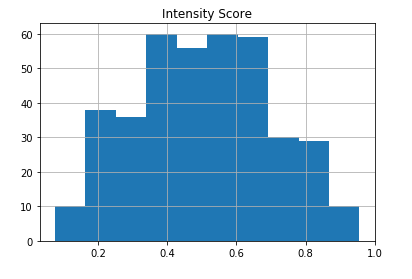
\includegraphics[width=\textwidth]{data_distrib.png}
\end{frame}

\section{Starting point}
\begin{frame}{Baseline entry point}
    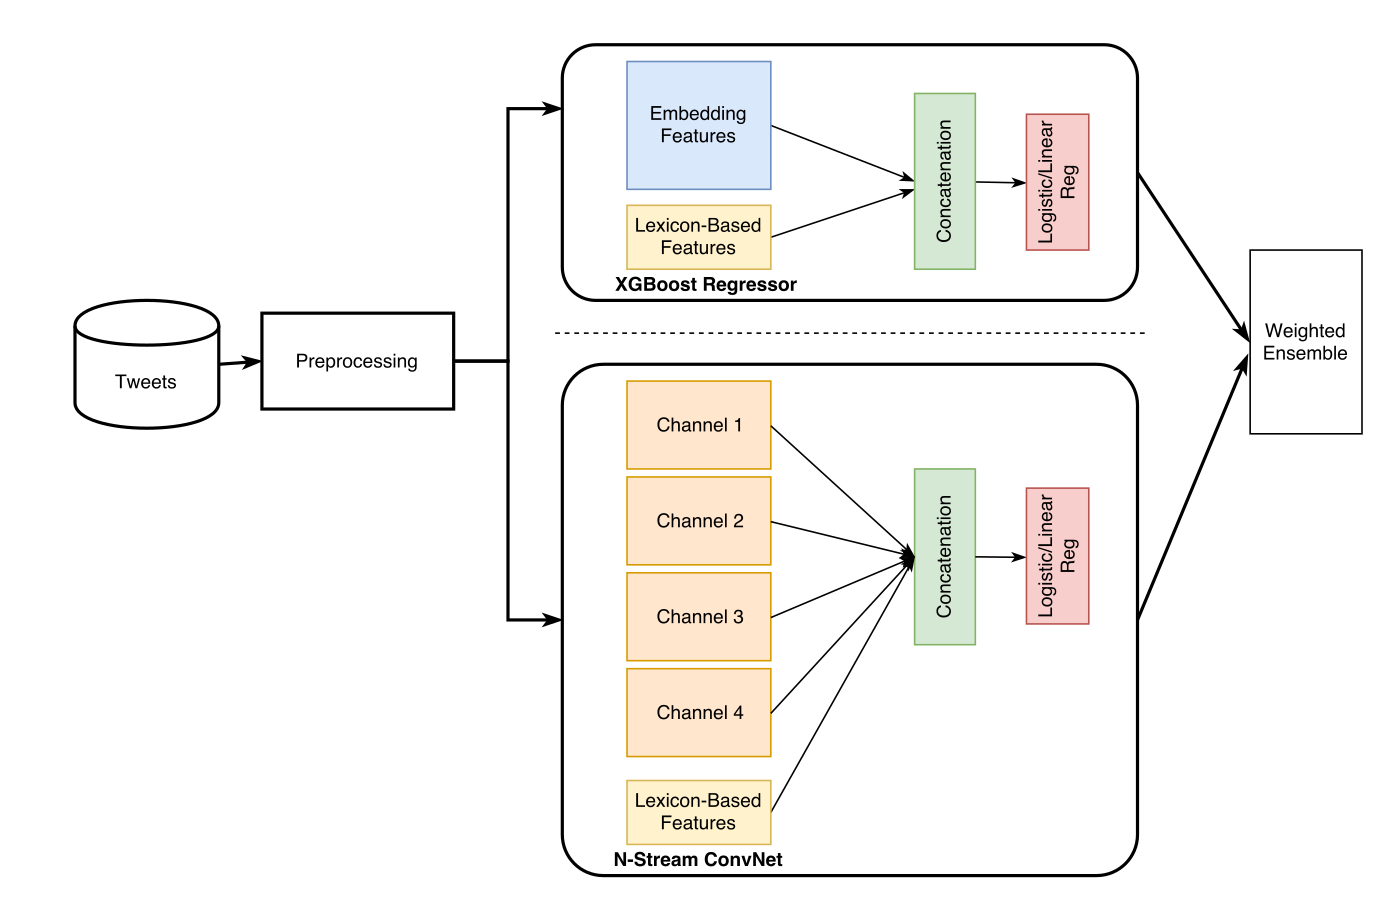
\includegraphics[width=\textwidth]{architecture.png}
\end{frame}

\end{document}
